
\minpurp{Suche im Array}
\minmeth{Sequentiell}
gehe der reihe nach alle elemente durch bis das element gefunden \textbf{O(n)}

\minmeth{Binär}
Sortiertes Array; betrachte mittleres Element; \\
<: Wiederhole im linken Teilarray, >: im rechten; worst-Case: \textbf{ $O(\log_2n)$}

\minmeth{Quick-Select}
Suche k. kleinstes element: Analog zu probab. Quicksort, betrachte nur das Teilarray, in dem der Index k liegt;  durchschnitt \textbf{O(n)}

\minpurp{Selection-Sort}
Suche Minimum; Tausche es mit dem ersten Element; Wiederhole im Array [2...n], \textbf{ O\{$n^2$\}}

\minpurp{Bubble-Sort}
durchlaufe elemente, tausche mit nachfolger wenn dieser größer; wiederhole \textbf{O\{$n^2$\}}

\minpurp{Quicksort}
\halfpage{\begin{enumerate}
\item Wähle Pivot= letztes Element
\item lasse zeiger von beiden Enden des Restarrays nach innen laufen: \\
 wenn der rechte zeiger auf ein kleineres bzw. der linke auf ein größeres Element als das Pivot zeigt stoppe den zeiger; wenn beide gestoppt: tausche sie, wenn sich die Zeiger treffen tausche das Pivot nach innen 
\item Wiederhole Quicksort im Rechten und linken Teilarray.
\end{enumerate}
}
Laufzeit: best Case:$O(n\log_2n)$, worst-Case $O(n^2)$

\submeth{probabilistisch:} start: wähle zufälliges Element als Pivot und tausche ans ende
\quarterpage{
\minpurp{Heapsort}
Interpretation Array als binärer Heap;\\
a[2i] und a[2i+1] sind die Kinder von a[i];\\
 Array durchläuft die Ebenen von oben nach unten, von links nach rechts

Heapbedingung: Vater $\leq$ Kinder
}
\quarterpage{
z.B. $[\underbrace{37}, \underbrace{45,57}, \underbrace{59,58, 99}] $=\\
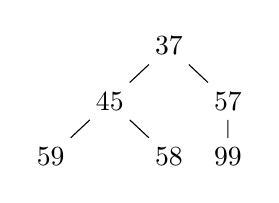
\begin{tikzpicture}[level distance=2em]
\node{37} 
child{ node{45}
child{ node{59}}
child{ node{58}}}
child{ node{57}
child{ node{99}}
}
;
\end{tikzpicture}
}

\minmeth{Heapsort}
Erzeuge Heap; 
Tausche letztes Element mit Wurzel, DownHeap in [1...n-1] , wiederhole bis array leer; 
worst-case: $O(n\log_2n)$

\minmeth{Erzeuge Heap}
Führe Einsichern für alle knoten durch (ebenenweise von unten rechts zur wurzel); \textbf{O(n)}

\minmeth{DownHeap}
Knoten > Kind: Tausche mit Kleinerem nachfolger; wiederhole rekursiv

\minmeth{Revisited}
Bestimme Pfad der kleineren Nachfolger bis zum Blatt, speichere den index.\\ 
=> index des i. Knotens auf dem Pfad sind die vordersten i Bits des Blattindex

\submeth{Lineare Suche:}
Suche vom Pfadende aus die Einfügestelle, speichere Wurzel, alle Pfadelemente rücken eine Ebene nach oben, einfügen Wurzel

\submeth{binärsuche:} analog dazu, suche Einfügestelle mit binärer Suche im Pfad 



